% Автор разбора: Антон Банных

\begin{frame}
  \frametitle{Задача <<Откат>>}
  \begin{center}
    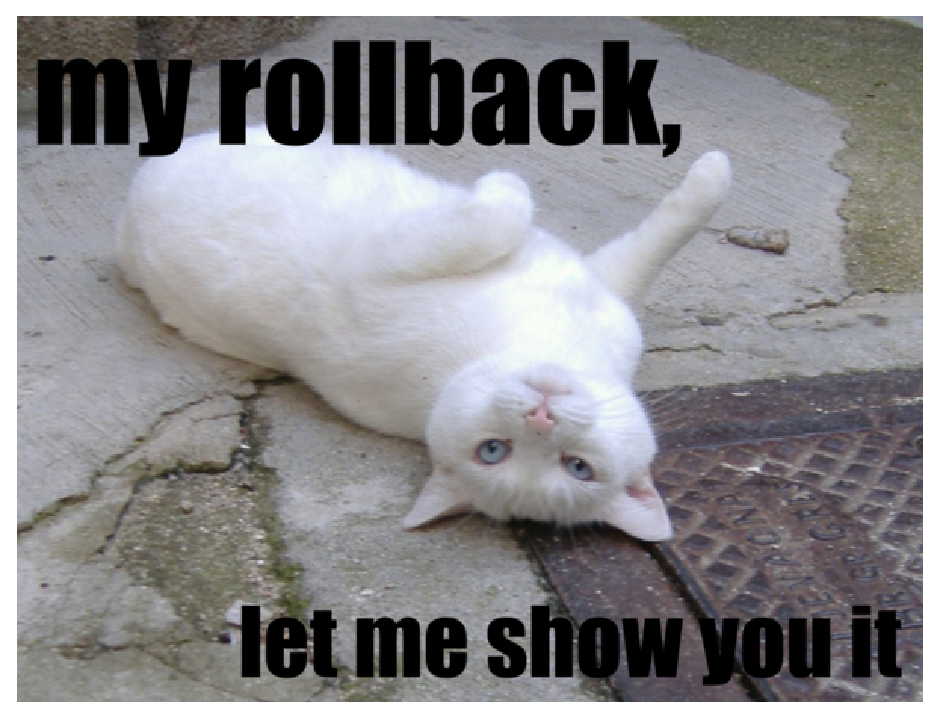
\includegraphics[width=10cm]{rollback.eps}
  \end{center}
\end{frame}

\begin{frame}
  \frametitle{Над задачей работали}
  \begin{itemize}
    \item Идея задачи: Антон Банных
    \item Текст условия: Антон Банных
    \item Тесты, проверяющая программа и др.: Антон Банных
    \item Решения: Антон Банных, Антон Ахи
    \item Текст разбора: Антон Банных
  \end{itemize}
\end{frame}

\begin{frame}
  \frametitle{Формулировка задачи}
  \begin{itemize}
    \item Дано $n$ целых чисел $a_1, a_2, \ldots, a_n$ и $q$ запросов
    \item Запрос~--- числа $l$ и $k$
    \item Ответ на запрос~--- минимальное число $r$, такое что $a[l..r]$ содержит $k$ различных чисел
    \item Онлайн-ответы на запросы
  \end{itemize}
\end{frame}

\begin{frame}
  \frametitle{Первый шаг решения}
  \begin{itemize}
    \item Упрощение: $l = 1$
    \item Пусть $b_i = 1$, если число $a_i$ не встречалось ранее
    \item В противном случае $b_i = 0$
    \item Ответ на запрос~--- минимальное $r$, такое что $\sum_{i=1}^r{b_i} = k$
    \item Построим дерево отрезков на сумму на массиве $b$
    \item Ответ на запрос за $O(\log n)$ при помощи <<спуска по дереву>>
      \begin{itemize}
        \item В вершине хранится сумма $sum$ на отрезке $[L..R]$                  
        \item В каждой вершине известно, куда идти (в лебого ребенка, или в правого)
      \end{itemize}
  \end{itemize}
\end{frame}

\begin{frame}
  \frametitle{Дальнейшее развитие идеи}
  \begin{itemize}
    \item Что делать, если $l=2$?
    \item Положим $b_1$ равным $0$
    \item Пусть $j$~--- первое вхождение $a_1$ в $a[2..n]$
    \item Положим $b_j$ равным $1$
    \item В массиве $b$ изменилось не более двух элементов
    \item Легко изменить дерево отрезков соответствующим образом
    \item Время на изменение $O(\log n)$
  \end{itemize}
\end{frame}


\begin{frame}
  \frametitle{Второй шаг}
  \begin{itemize}
    \item Умеем отвечать на запрос и переходит к следующему суффиксу за $O(\log n)$
    \item Предположим, что на запросы можно отвечать в произвольном порядке
    \item Отсортируем запросы по $l$
    \item Будем перебирать суффиксы в порядке уменьшения длины и отвечать на все запросы для данного суффикса
    \item Время работы $O(n \log n)$
    \item Используемая память O(n)
  \end{itemize}
\end{frame}

\begin{frame}
  \frametitle{Замечания по реализации}
  \begin{itemize}
    \item Для эффективного перехода необходимо для $i$-го символа знать первое вхождение числа $a_i$ в $a[i+1..n]$
    \item Идем слева направо
    \item Для каждого числа $c$ помним его последнее вхождение $d[c]$
    \item При обработке $a_i$ записываем его первое вхождение в $a[i+1..n]$ и обновляем $d[a_i] = i$
    \item Время работы $O(n)$
    \item Используемая память $O(n + m)$
    \item Можно совместить с основной частью, если перебирать суффиксы в порядке увеличения длины
  \end{itemize}
\end{frame}

\begin{frame}
  \frametitle{Решение основной задачи}
  \begin{itemize}
    \item Основная проблема "--- ответ на запрос <<онлайн>>
    \item Для сохранения всех деревьев отрезков потребуется слишком много памяти
    \item Наблюдение: при переходе к следующему суффиксу изменяется порядка $2 \log n$ вершин дерева отрезков
    \item Решение: персистентное дерево отрезков
  \end{itemize}
\end{frame}

\begin{frame}
  \frametitle{Персистентное дерево отрезков}
  \begin{itemize}
    \item Вместо изменения значения в вершине создаем новую
    \item Один запроc вида \texttt{set} создает $\log n$ вершин по пути от корня к листу.
    \item Старое дерево отрезков не меняется
    \item Новый корень соответствует измененному дереву отрезков
    \item Реализация запроса \texttt{get} не меняется
    \item Вызов $get$ от разных корней "--- все равно, что от разных деревьев
  \end{itemize}
\end{frame}

\begin{frame}
  \frametitle{Решение основной задачи}
  \begin{itemize}
    \item Переберем все суффиксы
    \item Для каждого суффикса запомним соответствующий корень дерева отрезков
    \item Для того, чтобы ответить на запрос вызываем \texttt{get} от соответствующего корня
    \item Время работы $O(n \log n)$
    \item Используемая память $O(n \log n + m)$
  \end{itemize}
\end{frame}

\begin{frame}
  \frametitle{Итого}
  \begin{itemize}
    \item Вопросы?
  \end{itemize}
\end{frame}